% Preambel
\documentclass[a4paper,openany]{report}


\usepackage{a4wide}
\usepackage[ansinew]{inputenc}
\usepackage[T1]{fontenc}
\RequirePackage{ifpdf}

\usepackage{hyperref}
	\hypersetup{%
  colorlinks=true,   % activates colored references
  pdfpagemode=None,  % PDF-Viewer starts without content et.al.
  pdfstartview=FitH, % PDF-Viewer uses a defined page width
  %linkbordercolor=111,
  % citebordercolor=111,
  citecolor=blue,
  linkcolor=blue}

\ifpdf
  \usepackage[pdftex]{graphicx}
	  \DeclareGraphicsExtensions{.pdf}
\else
  \usepackage[dvips]{graphicx}
	  \DeclareGraphicsExtensions{.eps}
\fi
	
\usepackage{fancyhdr}
\usepackage{booktabs}
%\usepackage[dvips]{rotating}
\usepackage{multirow}
\usepackage{multicol}

\usepackage{color}
\usepackage{amsmath}
\usepackage{alltt}
%\usepackage{array}
%\usepackage{colortbl}

\clubpenalty = 10000
\widowpenalty = 10000 \displaywidowpenalty = 10000

\definecolor{hellgrau}{gray}{0.95}
\definecolor{dunkelgrau}{gray}{0.55}



\renewcommand{\headrulewidth}{0pt} % no head rule
\renewcommand{\footrulewidth}{0pt} % no foot rule




%\nointend
%%%%%%%%%%%%%%%%%%%%%%%%%%%%%%
% start text here!!



\begin{document}
\pagenumbering{roman}

\title{A neural network toolbox for Octave\\
			Developer's Guide\\
			  Version: 0.1.9}

\author{M. Schmid}
\maketitle


\tableofcontents
\pagenumbering{arabic}

\chapter{Introduction}
This documentation isn't a well defined and structured docu for the neural network toolbox.
It's more a \textit{collection of my ideas and minds}.

\section{Installed system}
I'm developing and testing the actual version of the neural network toolbox on following 
program versions:

\begin{itemize}
  \item Octave 2.9.5
  \item octave-forge-2006.01.28
  \item OctPlot svn version
\end{itemize}


\section{Version numbers of the neural network toolbox}

The first number describes the major release. Version number V1.0 will be the first toolbox release which should have the same functions like the Matlab R14 SP3 neural network Toolbox.\\

The second number defines the finished functions. So to start, only the MLPs will realised and so this will be the number V0.1.0.\\

The third number defines the status of the actual development and function. V0.0.1 means no release with MLP, actually, everything under construction... ;-D.\\

Right now it's version V0.1.3 which means MLP works and currently the transfer function logsig is added.
\section{Code convention}

The main function of this toolbox will be programed with help of the book in \cite{4}.
So the variables will have the same names like in the book with one exception: Variables, only with one letter, will have two letters, e.g. 
\begin{itemize}
	\item $X \rightarrow Xx$
	\item $Q \rightarrow Qq$
	\item $a \rightarrow aa$
\end{itemize}
and so on ...\\

This is only to make it possible to search for variable names.

%\section{Varietes}
\label{chap:intro:sec:varietes}
\subsection{Object-oriented programming}
Some of the functions for Octave will have not the same name, like the matlab ones has.
This difference is because the object-oriented programming technology. The object-oriented functions will have a name postfix in Octave.\\
As example: \textit{isposint\_netw\_priv} means, \textit{isposint} is a private function from the matlab function \textit{network}.\\
This is a kind of "`simulation"' for the object-oriented programming technology.\\

\subsubsection{Data-Typ \textit{network} and m-file \textit{subsasgn}}
Matlab has a further data type \textit{network}. A basic neural network will be initialized in a
structure and than changed to the \textit{network} type with the \textit{class} command. The class command from Octave doesn't support the creation of this network type!
In the Matlab m-file \textit{network.m} on row 256, the network type will be created! From this moment, structure subscription assignment will call the file subsasgn from the \textit{@network} directory. Back in the \textit{newff} m-file on row 134, the @network subsasgn will be called the first time.

\paragraph{newff row 134; net.biasConnect} net=subsasgn(net,subscripts,v) will hold the following values:
\begin{itemize}
	\item net: the whole net structure
	\item subscripts: 1x1 structure;\\
		subscripts.type = '.'\\
		subscripts.subs = 'biasConnect'
	\item v: 2x1 double [1; 1]
\end{itemize}

\paragraph{newff row 135; net.inputConnect} net=subsasgn(net,subscripts,v) will hold the following values:
\begin{itemize}
	\item net: the whole net structure
	\item subscripts: 1x2 structure;\\
		subscripts(1).type = '.'\\
		subscripts(1).subs = 'inputConnect'\\
		subscripts(2).type = '()'\\
		subscripts(2).subs = [1] [1]
	\item v: 1x1 double 1
\end{itemize}
\textcolor{red}{bis hier sollte es erledigt sein...!}

\paragraph{newff row 137; net.layerConnect} net=subsasgn(net,subscripts,v) will hold the following values:
\begin{itemize}
	\item net: the whole net structure
	\item subscripts: 1x1 structure;\\
		subscripts(1).type = '.'\\
		subscripts(1).subs = 'layerConnect'
	\item v: 2x2 logical [0 0; 1 0]
\end{itemize}

\paragraph{newff row 138; net.outputConnect} net=subsasgn(net,subscripts,v) will hold the following values:
\begin{itemize}
	\item net: the whole net structure
	\item subscripts: 1x2 structure;\\
		subscripts(1).type = '.'\\
		subscripts(1).subs = 'outputConnect'\\
		subscripts(2).type = '()'\\
		subscripts(2).subs = '[2]'
	\item v: 1x1 double = 1
\end{itemize}

\paragraph{newff row 139; net.targetConnect} net=subsasgn(net,subscripts,v) will hold the following values:
\begin{itemize}
	\item net: the whole net structure
	\item subscripts: 1x2 structure;\\
		subscripts(1).type = '.'\\
		subscripts(1).subs = 'targetConnect'\\
		subscripts(2).type = '()'\\
		subscripts(2).subs = '[2]'
	\item v: 1x1 double = 1
\end{itemize}


\subsection{Data types}

\begin{table}
	\centering
	\begin{tabular}{c c c}
		\toprule
									& Matlab										& Octave\\
		\midrule
  								& double 											& double \\
									& int8  											& \\
									& int16 											& \\
									& int32 											& \\
									& int64 											& \\
			Numeric			& single											& \\
									& uint8 											& \\
									& uint16											& \\
									& uint32 											& \\ 
									& uint64 											& \\ 
									& complex 										& complex\\
		\midrule
			characters	& x														&  \\
		\midrule
			string			&															& \\
		\midrule
			cell				&	x														& x \\
		\midrule
			structure		& x 												  & x  \\
		\bottomrule
	\end{tabular}
\end{table}


\chapter{Octave}
This chapter describes all functions available in the neural network toolbox in Octave.
All the functions will be in two directorys till now. This will be: nnet/nnet/... and
nnet/nnutils/...

\section{Functions location}

\subsection{Directory \textit{nnet/nnet}}

\noindent Available functions:
\begin{enumerate}
	\item min\_max
	\item network
  \item newff
\end{enumerate}


\subsection{Directory \textit{nnet/nnutils}}
This directory holds a further subdirectory: \textit{saveMLPStructure}.\\

\noindent Available functions:
\begin{enumerate}
  \item saveMLPStruct
	
\end{enumerate}

Function \textit{saveMLPStruct} doesn't exist in MATLAB(TM). This is a helper function to print a neural network architecture.

\subsubsection{saveMLPStructure}
Inside this directory are a lot of different functions which will help to print a
text file to display the neural network architecture. The look will be the same like
you would open the type \textit{network} in MATLAB(TM).

\begin{itemize}
  \item printAdaptFcn
  \item printAdaptParam
  \item printB
  \item printBiasConnect
  \item printBiases
  \item printInitFcn
  \item printInputConnect
  \item printInputs
  \item printInputWeights
  \item printIW
  \item printLayerConnect
  \item printLayers
  \item printLayerWeights
  \item printLW
  \item printMLPHeader
  \item printNumInputDelays
  \item printNumInputs
  \item printNumLayerDelays
  \item printNumLayers
  \item printNumOutputs
  \item printNumTargets
  \item printOutputConnect
  \item printOutputs
  \item printPerformFcn
  \item printPerformParam
  \item printTargetConnect
  \item printTargets
  \item printTrainFcn
  \item printTrainParam
\end{itemize}

\section{Available functions}
\subsection{min\_max}
\textit{min\_max} get the minimal and maximal values of an training input matrix. So the dimension of this matrix must be an RxN matrix where R is the number of input neurons and N depends on the number of training sets.\\

\noindent \textbf{\textcolor{brown}{Syntax:}}\\

\noindent mMinMaxElements = min\_max(RxN);\\

\noindent \textbf{\textcolor{brown}{Description:}}\\

\noindent RxN: R x N matrix of min and max values for R input elements with N columns\\ 

\noindent \textbf{\textcolor{brown}{Example:}}\\

\begin{equation}
	\left[
		\begin{array}{cc}
     	1 &  11 \\
    	0  & 21
   \end{array} 
	 \right]            = min\_max\left[ 
	 															   \begin{array}{ccccc}
	 															   3 & 1 & 3 & 5 & 11 \\
	 															   12& 0 & 21& 8 & 6  \\
	 															   \end{array}
	 															   	 \right]
\end{equation}


\chapter{Coding Guideline}
Some genereal descriptions why a variable has a chosen name. This is valid for the complete
toolbox... or so :-)\\
Here is only the description of variable names, which aren't visible to the user. Visible names are
described in the User's Guide!\\
The variable identifiers are taken from \cite{4}. One difference is purposeful added. If a variable has only one letter, a second small letter will be added to make it searchable. Who has ever tried to search a variable called "t"?

\section{Variable identifier}

\begin{tabbing}
\hspace*{1em} \= \textcolor{blue}{Identifier} \hspace*{3em}\= \textcolor{blue}{Description:} \\ 
  \textbf{Aa} \> \> hold the network values after transfer function.\\
  blf \>  \> \textbf{b}atch \textbf{l}earning \textbf{f}unction \\
  btf  \>  \> \textbf{b}atch \textbf{t}rainings \textbf{f}unction \\
  \textbf{Jj} \>  \> Jacobi matrix \\
  \textbf{Nn}  \> \> hold the network values before transfer function.\\  						
  net	\> \> structure which holds the neural network informations \\
  pf \>  \> \textbf{p}erformance \textbf{f}unction \\
  \textbf{Pp}				\>						\>input matrix; nInputs x nDataSets  \\
  \textbf{Pr}	\>		\> input range, this is a Nx2 matrix, that's why the capitalized P \\
  trf \>  \> \textbf{tr}ansfer \textbf{f}unction \\
  \textbf{Tt} \>  \> target matrix, nTargets x nDataSets\\
  \textbf{ss}	\> \> row vector with numbers of neurons in the layers, for each layer, one entry \\
  \textbf{vE}	\> \> row vector with errors... size depends on network structure. \\
  VV \>  \> Validation structure \\
  \textbf{xx} \>  \> Weight vector in column format\\
  
\end{tabbing}

\subsection{Nn}
\textbf{Nn} is a cell array and has one entry for each layer. This means in the actual allowed network
structure, 2 entries.\\
In \textbf{Nn\{1,1\}} are the values for the first (and only) hidden layer. The size of this matrix depends
on the number of neurons used for this layer.\\
In \textbf{Nn\{2,1\}} are the values for the output layer. The size of this matrix depends
on the number of neurons used for this layer.\\

\subsection{Aa}
\textbf{Aa} is a cell array and has one entry for each layer. This means in the actual allowed network
structure, 2 entries.\\
In \textbf{Aa\{1,1\}} are the values for the first (and only) hidden layer. The size of this matrix depends
on the number of neurons used for this layer.\\
In \textbf{Aa\{2,1\}} are the values for the output layer. The size of this matrix depends
on the number of neurons used for this layer.\\

\subsection{vE}
\textbf{vE} is also a cell array which holds (till now) in the second element the error vector. It's not completly clear, why in the second element.\\
The number of rows depends on the number of output neurons. For one output neuron, \textbf{vE} holds only one row, for 2 output neurons, this holds of course 2 rows. 

\subsection{Jj}
This is the short term for the Jacobi matrix.
\chapter{Algorithm}
Here are some general thoughts about calculating parts are used in algorithm.

\section{Levenberg Marquardt}
This algorithm will be programed with \cite{4}.

\subsection{Sensitivity Matrix}
How does this looks like?\\
\begin{enumerate}
	\item for a 1-1-1 MLP
	\item for a 2-1-1 MLP
	\item for a 1-2-1 MLP
\end{enumerate}

\subsubsection{1-1-1 MLP}
In this case, the MLP holds one input neuron, one hidden neuron and one output neuron. The number of weights needed for this MLP is 4 (2 weights, 2 biases).\\

It needs two sensitivity matrices because the two layers. Each sensitivity matrix will hold 1 element.
This is taken from \cite{4}, example P12.5 page 12-44. Attention, in this example are two data sets used, this is the reason for the 4 elements...!

\subsubsection{2-1-1 MLP}
In this case, the MLP holds two input neurons, one hidden neuron and one output neuron. The number of weights needed for this MLP is 5 (3 weights, 2 biases).\\

It needs also two sensitivity matrices because the two layers. Actually, the input is not only a scalar, it is a vector with 2 elements. Even though, again after \cite{4}. I think the sensitivity matrices will hold only 1 element. So the number of elements will bi proportional to the number of hidden neurons and the number of output neurons.

\subsubsection{1-2-1 MLP}
In this case, the MLP holds one input neuron, two hidden neurons and one output neuron. The number of weights needed for this MLP is 7 (4 weights, 3 biases).\\

It needs also two sensitivity matrices because the two layers. Actually, the input is again only a scalar. 
Now calculating $n_1^1$ will result in a row vector with 2 elements. $n_1^2$ will hold only one element and so we have 3 elements in the sensitivity matrix.\\

We can say, the number of hidden neurons is responsible for the dimension of the sensitivity matrices.
For example, a 4-3-1 MLP with 100 data sets will generate following sensitivity matrix for the first layer:
$\tilde{\textbf{S}}^1 = [\tilde{\textbf{S}}^1_1 | \tilde{\textbf{S}}^1_2 | ... | \tilde{\textbf{S}}^1_{100}]$\\
\noindent $\tilde{\textbf{S}}^1_1$ will hold 3 elements  $\tilde{\textbf{S}}^1_1 = [\tilde{\textbf{S}}^1_{1,1} ~ \tilde{\textbf{S}}^1_{2,1} ~ \tilde{\textbf{S}}^1_{3,1}]^T$;
$\tilde{\textbf{S}}^1_2 = [\tilde{\textbf{S}}^1_{1,2} ~ \tilde{\textbf{S}}^1_{2,2} ~ \tilde{\textbf{S}}^1_{3,2}]^T$ and so on. So matrix will have a size of 3x100 for $\tilde{\textbf{S}}^1_{1}$
and a size of 1x100 for $\tilde{\textbf{S}}^1_{2}$.\\

By the way, the jacobian matrix will be a 100x20 matrix ..






\chapter{Test}

\section{isposint}
\begin{verbatim}
%!shared
%! disp("testing isposint")
%!assert(isposint(1)) # this should pass
%!assert(isposint(0.5),0) # should return zero
%!assert(isposint(-1),0) # should return zero
%!assert(isposint(-1.5),0) # should return zero
%!assert(isposint(0),0) # should return zero
%!fail("isposint([0 0])","Input argument must not be a vector, only scalars are allowed!")
%!fail("isposint('testString')","Input argument must not be a vector, only scalars are allowed!")
\end{verbatim}

\section{min\_max}
\subsection{min\_max}
\textit{min\_max} get the minimal and maximal values of an training input matrix. So the dimension of this matrix must be an RxN matrix where R is the number of input neurons and N depends on the number of training sets.\\

\noindent \textbf{\textcolor{brown}{Syntax:}}\\

\noindent mMinMaxElements = min\_max(RxN);\\

\noindent \textbf{\textcolor{brown}{Description:}}\\

\noindent RxN: R x N matrix of min and max values for R input elements with N columns\\ 

\noindent \textbf{\textcolor{brown}{Example:}}\\

\begin{equation}
	\left[
		\begin{array}{cc}
     	1 &  11 \\
    	0  & 21
   \end{array} 
	 \right]            = min\_max\left[ 
	 															   \begin{array}{ccccc}
	 															   3 & 1 & 3 & 5 & 11 \\
	 															   12& 0 & 21& 8 & 6  \\
	 															   \end{array}
	 															   	 \right]
\end{equation}


\section{newff}
\subsection{newff}
\textit{newff} is the short form for \textit{\textbf{new f}eed \textbf{f}orward network}. This command creates a feed-forward backpropagation network structure.\\

\noindent \textbf{\textcolor{brown}{Syntax:}}\\

\noindent net = newff(Rx2,[S1 S2 ... SN],\{TF1 TF2 ... TFN\},BTF,BLF,PF)\\

\noindent \textbf{\textcolor{brown}{Description:}}\\

\noindent Rx2: R x 2 matrix of min and max values for R input elements\\ 
\noindent Si: Size of ith layer, for N layers\\ 
\noindent TFi: Transfer function of ith layer, default = "tansig"\\
\noindent BTF: Backpropagation network training function, default = "trainlm" \\
\noindent BLF: Backpropagation weight/bias learning function, NOT USED, is only for MATLAB(TM) compatibility\\
\noindent PF: Performance function, default = "mse"\\

\noindent \textbf{\textcolor{brown}{Examples:}}\\

\noindent net = newff(Rx2,[2 1])\\
\noindent net = newff(Rx2,[2 1],\{"tansig","purelin"\});\\
\noindent net = newff(Rx2,[2 1],\{"tansig","purelin"\},"trainlm");\\
\noindent net = newff(Rx2,[2 1],\{"tansig","purelin"\},"trainlm","notUsed","mse");\\

\noindent \textbf{\textcolor{brown}{Comments:}}\\
In this version, you can have as much output neurons as you want. The same with the number of hidden layers. This means you can have one input layer, unrestricted number of hidden layers and one output layer. That's it.\\



\section{prestd}
\subsection{min\_max}
Checks for minimal and maximal values of an input matrix for \textbf{newff}.\\

\subsubsection{Syntax:}

$pr = min\_max(mInputs)$\\

\subsubsection{Description:}
\textit{mInputs} must be a matrix with input training data sets. This means in the case, for a 9-2-1 MLP
(this means 9 input-, 2 hidden- and 1 output-neuron) with 100 input training data sets, the matrix must be
an 9x100 matrix. \textit{pr} will then be a 9x2 matrix with minimal values in the first column and maximal values in the second column. If a row holds 2 zeros, a warning will appear (no information in this row!).

\subsubsection{Important:}
The equival function in MATLAB(TM) is called \textit{minmax}. This is not possible because the functions \textit{min} and \textit{max} in Octave are programed in minmax.cc!
\section{purelin}
\subsection{purelin}

\begin{figure}[htb]
\centering
  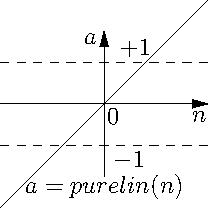
\includegraphics{octave/neuroPackage/graphics/purelin}
\caption{Linear transfer function}
\label{fig:purelinTransferFunction}
\end{figure}

\begin{figure}[htb]
\centering
  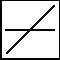
\includegraphics{octave/neuroPackage/graphics/purelinlogo}
\caption{Linear transfer function logo}
\label{fig:purelinTransferFunctionLogo}
\end{figure}


\section{subset}
\subsection{subset}

\textit{subset} can be used to optimize the data sets for train, test and validation of a neural
network.\\

\noindent \textbf{\textcolor{brown}{Syntax:}}\\

\noindent [mTrain, mTest, mVali] = subset(mData,nTargets,iOpti,fTest,fVali);\\

\noindent \textbf{\textcolor{brown}{Description:}}\\

\noindent  \textbf{Left-Hand-Side:}\\
\noindent mTrain: (R+T) x M matrix with R input rows, T output rows and M columns
				where M <= N.\\
\noindent mTest:  (R+T) x S matrix with R input rows, T output rows and S columns
				where S <= N.\\
\noindent mVali:  (R+T) x U matrix with R input rows, T output rows and U columns
				where U <= N. And U can only exist, if S also exist.\\

\noindent  \textbf{Right-Hand-Side:}\\
\noindent mData: (R+T) x N matrix with R input rows, T output rows and N columns\\ 
\noindent nTargets: Number of T output rows\\ 
\noindent iOpti: Integer value to define level of optimization.\\
\noindent fTest: Fraction to define the percentage of data sets which should be used for testing. \\
\noindent fVali: Fraction to define the percentage of data sets which should be used for testing.\\

\noindent iOpti can have following values:\\
0	: no optimization\\
1	: will randomise the column order and rerange the columns containing min and max values to be in the train set\\
2	:	will NOT randomise the column order, but rerange the columns containing min and max values to be in the train set\\

\noindent fTest or fValie have following meaning:\\
Each of this arguments can be a fraction or zero. The value 1 is not allowed! The sum of both values
must also be smaller than 1!\\
Example: fTest = 1/3\\

\noindent \textbf{Default values}\\
\noindent iOpti		= 1\\
\noindent fTest		= 1/3\\
\noindent fVali		= 1/6\\

\noindent \textbf{\textcolor{brown}{Examples:}}\\

\noindent mTrain = subset(mData,2,1,0,0)\\
\noindent [mTrain,mTest] = subset(mData,2,1,1/3,0);\\
\noindent [mTrain,mTest,mVali] = subset(mData,1);\\
\noindent [mTrain,mTest,mVali] = subset(mData,1,1,1/3,1/6);\\
\section{\_\_analyzerows}
\begin{verbatim}
%!shared b, retmat
%! disp("testing __analyzerows")
%! b = [1 0 0 1; 1 0 0 0; 1 2 0 1];
%! retmat = __analyzerows(b);
%!assert(retmat(1,1)==1);#%!assert(retmat(1,1)==1);
%!assert(retmat(2,1)==1);
%!assert(retmat(3,1)==0);
%! b = [1 0 0 2; 1 0 0 0; 1 1 1 1];
%! retmat = __analyzerows(b);
%!assert(retmat(1,2)==0);
%!assert(retmat(2,2)==0);
%!assert(retmat(3,2)==1);
%! b = [1 0 0 2; 1 0 0 0; 1 1 1 1];
%! retmat = __analyzerows(b);
%!assert(retmat(1,3)==2);
%!assert(retmat(2,3)==0);
%!assert(retmat(3,3)==0);
%! retmat = __analyzerows(b);
%!assert(retmat(1,4)==1);
%!assert(retmat(2,4)==0);
%!assert(retmat(3,4)==0);
\end{verbatim}

\section{\_\_copycoltopos1}
\begin{verbatim}
%!shared a, retmat
%! disp("testing __copycoltopos1")
%! a = [0 1 2 3 4; 5 6 7 8 9];
%! retmat = __copycoltopos1(a,3);
%!assert(retmat(1,1)==2);
%!assert(retmat(2,1)==7);
%! retmat = __copycoltopos1(a,5);
%!assert(retmat(1,1)==4);
%!assert(retmat(2,1)==9);
\end{verbatim}

\section{\_\_optimizedatasets}
\begin{verbatim}
%!shared retmatrix, matrix
%! disp("testing __optimizedatasets")
%! matrix = [1 2 3 2 1 2 3 0 5 4 3 2 2 2 2 2 2; \
%!			 0 1 1 0 0 0 0 0 0 0 0 0 0 0 1 1 0; \
%!			-1 3 2 4 9 1 1 1 1 1 9 1 1 1 9 9 0; \
%!			 2 3 2 3 2 2 2 2 3 3 3 3 1 1 1 1 1];
%! ## The last row is equal to the neural network targets
%! retmatrix = __optimizedatasets(matrix,9,1);
%! ## the above statement can't be tested with assert!
%! ## it contains random values! So pass a "success" message
%!assert(1==1);
%! matrix = [1 2 3 2 1 2 3 0 5 4 3 2 2 2 2 2 2; \
%!			 0 1 1 0 0 0 0 0 0 0 0 0 0 0 1 1 0; \
%!			-1 3 2 4 9 1 1 1 1 1 9 1 1 1 9 9 0; \
%!			 2 3 2 3 2 2 2 2 3 3 3 3 1 1 1 1 1];
%! ## The last row is equal to the neural network targets
%! retmatrix = __optimizedatasets(matrix,9,1,0);
%!assert(retmatrix(1,1)==5);
%!assert(retmatrix(2,1)==0);
%!assert(retmatrix(3,1)==1);
%!assert(retmatrix(4,1)==3);
\end{verbatim}

\section{\_\_randomisecols}
\begin{verbatim}
%!# no test possible, contains randperm which is using
%!# some randome functions
\end{verbatim}

\section{\_\_rerangecolumns}
\begin{verbatim}
%!shared matrix,analyzeMatrix,nTrainSets, returnmatrix
%! disp("testing __rerangecolumns")
%! matrix = [0 1 0 0 0 0 1 0 1 1;  \
%!			 4 4 4 4 4 4 4 4 4 4;  \
%!        -1.1 -1.1 2 3 4 3.2 1 8 9 10; \
%!           0 1.1 3 4 5 2 10 10 2 3; \
%!          -1 1 1 1 1 2 3 4 1 5];
%! analyzeMatrix = [1 0 0 0; 0 1 0 0; 0 0 2 1; 0 0 1 2; 0 0 1 1];
%! nTrainSets = 8;
%! returnmatrix = __rerangecolumns(matrix,analyzeMatrix,nTrainSets);
%!assert(returnmatrix(1,1)==1);
%!assert(returnmatrix(2,1)==4);
%!assert(returnmatrix(3,1)==1);
%!assert(returnmatrix(4,1)==10);
%!assert(returnmatrix(5,1)==3);
%! matrix = [0 1 0 0 0 0 1 0 1 1; 			\
%!			 4 4 4 4 4 4 4 4 4 4; 			\
%!          -1.1 -1.1 2 3 4 3.2 1 8 9 10; 	\
%!           0 1.1 3 4 5 2 10 10 2 3; 		\
%!          -1 1 1 1 1 2 3 4 1 5;     		\
%!			 0 1 2 1 2 1 2 3 4 5;];  # the last row is euqal to the nnet targets
%! analyzeMatrix = [1 0 0 0; 0 1 0 0; 0 0 2 1; 0 0 1 2; 0 0 1 1];
%! nTrainSets = 8;
%! returnmatrix = __rerangecolumns(matrix,analyzeMatrix,nTrainSets);
%!assert(returnmatrix(1,1)==1);
%!assert(returnmatrix(2,1)==4);
%!assert(returnmatrix(3,1)==1);
%!assert(returnmatrix(4,1)==10);
%!assert(returnmatrix(5,1)==3);
%!assert(returnmatrix(6,1)==2);
\end{verbatim}


\chapter{analyzing matlab functions}

\section{analyzing newff}
First, \textit{newff} will be analyzed for a X-X-X mlp. This means, maximum 3 layers, including the input layer. Or in words, one input- one hidden- and one output-layer. The number of neurons are choosable.

Following command will be used, to create a new feed-forward neural network:\\
\noindent MLPnet = newff(mMinMaxElements,[nHiddenNeurons nOutputNeurons],...\newline
\{'tansig','purelin'\},'trainlm','learngdm','mse');\\

newff is the matlab command, mMinMaxElements is a $Rx2$-Matrix with minimum and maximum values of the inputs. $R$ is equal to the number of input neurons. [nHiddenNeurons nOutputNeurons] are the scalar values, to define the number of neurons in the hidden and output layer. One value, for each layer. \{'tansig','purelin'\} are the transfer functions, for each layer. This means, 'tansig' for the hidden layer and 'purelin' for the output layer. 'trainlm' is the training algorithm, in this case, Levenberg-Marquardt. 'learngdm' is the learn algorithm and 'mse' is the performance function, \textbf{m}ean-\textbf{s}quare-\textbf{e}rror.\\
MLPnet will be a structure with following content:

\begin{verbatim}
Neural Network object:

    architecture:

         numInputs: 1
         numLayers: 2
       biasConnect: [1; 1]
      inputConnect: [1; 0]
      layerConnect: [0 0; 1 0]
     outputConnect: [0 1]
     targetConnect: [0 1]

        numOutputs: 1  (read-only)
        numTargets: 1  (read-only)
    numInputDelays: 0  (read-only)
    numLayerDelays: 0  (read-only)

    subobject structures:

            inputs: {1x1 cell} of inputs
            layers: {2x1 cell} of layers
           outputs: {1x2 cell} containing 1 output
           targets: {1x2 cell} containing 1 target
            biases: {2x1 cell} containing 2 biases
      inputWeights: {2x1 cell} containing 1 input weight
      layerWeights: {2x2 cell} containing 1 layer weight

    functions:

          adaptFcn: 'trains'
           initFcn: 'initlay'
        performFcn: 'mse'
          trainFcn: 'trainlm'

    parameters:

        adaptParam: .passes
         initParam: (none)
      performParam: (none)
        trainParam: .epochs, .goal, .max_fail, .mem_reduc, 
                    .min_grad, .mu, .mu_dec, .mu_inc, 
                    .mu_max, .show, .time

    weight and bias values:

                IW: {2x1 cell} containing 1 input weight matrix
                LW: {2x2 cell} containing 1 layer weight matrix
                 b: {2x1 cell} containing 2 bias vectors

    other:

          userdata: (user stuff)
\end{verbatim}
\textit{numInputs: 1}: one input layer\\
\noindent \textit{numLayers: 2}: one hidden and one output layer\\
\noindent \textit{biasConnect: [1; 1]}: unknown till now!!\\
\noindent \textit{inputConnect: [1; 0]}: unknown till now!!\\
\noindent \textit{layerConnect: [0 0; 1 0]}: unknown till now!!\\
\noindent \textit{outputConnect: [0 1]}: unknown till now!!\\
\noindent \textit{targetConnect: [0 1]}: unknown till now!!\\
\noindent \textit{numOutputs: 1  (read-only)}: unknown till now!!\\
\noindent \textit{numTargets: 1  (read-only)}: unknown till now!!\\
\noindent \textit{numInputDelays: 0  (read-only)}: unknown till now!!\\
\noindent \textit{numLayerDelays: 0  (read-only)}: unknown till now!!\\
\noindent \textit{inputs: {1x1 cell} of inputs}: input layer definition\\
Because we have defined only one input layer, you can see the detailed definition with
following command in the matlab prompt:\\
\begin{verbatim}
	MLPnet.inputs{1}

ans = 

       range: [26x2 double]
        size: 26
    userdata: [1x1 struct]
\end{verbatim}
range are the min. and max. values of the inputs. size is the number of input neurons and userdata are user specified inputs...!\\
\noindent \textit{layers: {2x1 cell} of layers}: hidden and output layer definition\\
The dimension of $2x1 cell$ is because we have one hidden and one output layer. So too see the details of the hidden layer definitions, we have to enter:
\begin{verbatim}
K>> MLPnet.layers{1}

ans = 

     dimensions: 2
    distanceFcn: ''
      distances: []
        initFcn: 'initnw'
    netInputFcn: 'netsum'
      positions: [0 1]
           size: 2
    topologyFcn: 'hextop'
    transferFcn: 'tansig'
       userdata: [1x1 struct]
\end{verbatim}
and for the output layer:
\begin{verbatim}
K>> MLPnet.layers{2}

ans = 

     dimensions: 1
    distanceFcn: ''
      distances: []
        initFcn: 'initnw'
    netInputFcn: 'netsum'
      positions: 0
           size: 1
    topologyFcn: 'hextop'
    transferFcn: 'purelin'
       userdata: [1x1 struct]
\end{verbatim}

\noindent \textit{outputs: {1x2 cell} containing 1 output}: output layer definitions\\
\begin{verbatim}
K>> MLPnet.outputs

ans = 

     []    [1x1 struct]
\end{verbatim}
How knows, why this is a $1x2 cell$? The next command will also show the detailed definition! Of course, realy simple.
\begin{verbatim}
K>> MLPnet.outputs{2}

ans = 

        size: 1
    userdata: [1x1 struct]
\end{verbatim} 

\noindent \textit{targets: {1x2 cell} containing 1 target}: unknow till now\\

\noindent \textit{biases: {2x1 cell} containing 2 biases}: detailed definitions, for the biases\\
\begin{verbatim}
K>> MLPnet.biases

ans = 

    [1x1 struct]
    [1x1 struct]

K>> MLPnet.biases{1}

ans = 

       initFcn: ''
         learn: 1
      learnFcn: 'learngdm'
    learnParam: [1x1 struct]
          size: 2
      userdata: [1x1 struct]

K>> MLPnet.biases{2}

ans = 

       initFcn: ''
         learn: 1
      learnFcn: 'learngdm'
    learnParam: [1x1 struct]
          size: 1
      userdata: [1x1 struct]
\end{verbatim}
      inputWeights: {2x1 cell} containing 1 input weight
      layerWeights: {2x2 cell} containing 1 layer weight


\paragraph{weight and bias values:}

\subparagraph{IW:}
\begin{verbatim}
K>> MLPnet.IW

ans = 

    [2x26 double]
               []
\end{verbatim}

\subparagraph{LW:}
\begin{verbatim}
K>> MLPnet.LW

ans = 

              []     []
    [1x2 double]     []
\end{verbatim}

\subparagraph{b:}
\begin{verbatim}
K>> MLPnet.b

ans = 

    [2x1 double]
    [   -0.3908]
\end{verbatim}


\paragraph{net.trainParam:}
Output for the Levenberg-Marquardt train algorithm.
\begin{verbatim}
K>> MLPnet.trainParam

ans = 

       epochs: 100
         goal: 0
     max_fail: 5
    mem_reduc: 1
     min_grad: 1.0000e-010
           mu: 0.0010
       mu_dec: 0.1000
       mu_inc: 10
       mu_max: 1.0000e+010
         show: 25
         time: Inf
\end{verbatim}


\appendix
\chapter{Examples}


\section{Example 1}

This MLP is designed with 2-2-1. This is not a complete example but it will help to understand the
dimensions of all matrices and vectores are used inside the Levenberg-Marquardt algorithm.

\subsection{Data matrices}
The input matrix will be defined like in equation \eqref{equ:mInput} and the output matrix like in 
equation \eqref{equ:mOutput}.

\begin{equation}
  mInput = \left[ \begin{array}{c c c c}
												1 & 2 & 3 & 1   \\
												1	& 1 & 1 & 2 	\\
												1 & 2 & 1 & 2		\\																					
												\end{array}
					\right]
		\label{equ:mInput}
\end{equation}

\begin{equation}
  mOutput = \left[ \begin{array}{c c c c}
												1 & 1.5 & 2 & 3   \\																					
									 \end{array}
					\right]
		\label{equ:mOutput}
\end{equation}




\subsection{Weight matrices}
The first layer matrix will hold 2x3 weights. The second layer matrix will hold 1x2 weights.
The first bias holds 3x1 weights and the second holds only a scalar element.

\subsection{Sensitivity Matrices}
This part is right now not so clear in my mind. What is the dimension of these two matrices?
The first layer sensitivity matrix should be about 2x71. Number of hidden neurons in the rows and number of train data sets in the columns.\\

In the actual version, the dimension is about 71x71 .. so it seems to have a mistake inside the algorithm :-(


% Preamble

%\documentclass[a4paper]{report}

%\usepackage[ngerman]{babel}
%\usepackage[T1]{fontenc}
%\usepackage[ansinew]{inputenc}


%%%%%%%%%%%%%%%%%%%%%%%%%%%%%%
% start text here!!

%\begin{document}

\begin{thebibliography}{XXXXXXX}

\bibitem [1]{1} John W. Eaton

GNU Octave Manual, Edition 3, PDF-Version, February 1997

\bibitem [2]{2} The MathWorks, Inc.

MATLAB Online-Help

\bibitem [3]{3} Steven W. Smith

The Scientist and Engineer's Guide to Digital Signal Processing
ISBN 0-9660176-3-3, California Technical Publishing, 1997

\bibitem [4]{4} Martin T. Hagan, Howard B. Demuth, Mark Beale

Neural Network Design, ISBN 0971732108, PWS Publishing Company, USA, Boston, 1996





\end{thebibliography}
%\end{document}



\end{document}


